\documentclass[conference]{IEEEtran}
\usepackage{amsmath,amssymb,amsfonts}
\usepackage{graphicx}
\usepackage{booktabs}
\usepackage{cite}
\usepackage{url}
\usepackage{textcomp}
\usepackage{xcolor}
\usepackage{tikz}
\usepackage{pgfplots}
\pgfplotsset{compat=1.18}
\usetikzlibrary{arrows.meta, positioning, shapes.geometric, fit, backgrounds, calc, patterns}
\usepackage{hyperref}
\usepackage{multirow}
\usepackage{enumitem}

\begin{document}

\title{Embedding-Based Binary Classification of Person and
Merchant Names in Indian UPI Transactions Using
Attention-Enhanced MLP}

\author{
  \IEEEauthorblockN{[Authors]}
}

\maketitle

\begin{abstract}
Automated credit underwriting from Indian bank statements hinges on a deceptively simple question: is a given UPI counterparty a person or a business? Answering it is harder than it seems. Indian payee names are short, lack standardised formatting, and are often linguistically ambiguous---``Tanishq,'' for instance, is both a common given name and one of India's largest jewellery brands.

We tackle this with a two-stage pipeline. First, each payee string is encoded into a 1024-dimensional vector by Qwen3-Embedding-0.6B. Then an AttentionMLP classifier---which reshapes the embedding into 64 pseudo-tokens and applies multi-head self-attention---makes the binary decision. Trained on 233{,}478 synthetically generated Indian names, AttentionMLP reaches \textbf{98.4\%} test accuracy (F1\,$=$\,0.985, AUC\,$=$\,0.997), outperforming eight baselines that include SVMs, gradient-boosted trees, and deep MLPs. On a hand-curated set of deliberately ambiguous names it scores 85.4\%, and on fully unseen names 94.1\%. For deployment, the classifier exports to ONNX at just 10\,KB---205$\times$ smaller than the PyTorch checkpoint---and runs 9.5$\times$ faster on CPU. The complete pipeline, embedding model included, needs no PyTorch at inference time.
\end{abstract}

\begin{IEEEkeywords}
Merchant Classification, UPI Transactions, Text Embeddings, Self-Attention, ONNX Deployment
\end{IEEEkeywords}

%% -----------------------------------------------------------
\section{Introduction}
\label{sec:intro}

Every month, India's Unified Payments Interface (UPI) handles upward of 17~billion transactions~\cite{rbi2025vision}. Each one carries a narration string---a short, free-text field that names the counterparty. For a lender building a credit profile, that string is a goldmine: knowing that an applicant regularly pays Swiggy, BigBasket, or HDFC Life paints a far richer picture of spending behaviour than an account balance ever could~\cite{byanjankar2021predicting}.

Extracting value from these strings, however, is a multi-step process. The CreditMitra pipeline tackles it in three stages~\cite{dpqlora_paper}. In the first, a fine-tuned small language model pulls payee names from raw narration text. In the second---the focus of this paper---each extracted name is labelled as either an \emph{individual} (a person-to-person, or P2P, transfer) or a \emph{business} (a person-to-merchant, P2M, payment). In the third, merchant-level data feeds into structured credit-risk models.

Why is the second step so hard? Three reasons stand out. First, the names are short---often just one to three words---so there is very little lexical signal to work with. Second, many Indian brands borrow from personal names. ``Haldiram'' started as a founder's name; ``Tanishq'' doubles as a popular girl's name and a jewellery empire. These overlaps create genuine ambiguity. Third, formatting varies wildly across banks: the same merchant might appear in uppercase, title case, truncated, or prefixed with a UPI rail identifier.

Simpler approaches struggle here. Rule-based systems (keyword lists, suffix matching) break down precisely on the ambiguous boundary cases that matter most~\cite{nadeau2007ner_survey}. Prompting a large language model works but is far too slow for high-throughput pipelines~\cite{brown2020gpt3}. We take a middle path: encode each name into a dense embedding, then classify with a lightweight neural network.

Our contributions are fourfold:
\begin{enumerate}[leftmargin=*]
  \item A large-scale dataset of 233{,}478 Indian individual and business names, augmented to reflect real UPI formatting quirks.
  \item An extensive embedding-space analysis---UMAP, t-SNE, Fisher discriminant ratios, dimension ablation---that characterises where and why the two classes separate.
  \item AttentionMLP, a classifier that re-interprets a flat 1024-dim embedding as a token sequence and applies multi-head self-attention, reaching 98.4\% accuracy across nine baselines.
  \item A production-ready ONNX export that drops all PyTorch dependencies while preserving numerical equivalence.
\end{enumerate}

%% -----------------------------------------------------------
\section{Related Work}
\label{sec:related}

\subsection{Text Embeddings for Classification}

Dense text embeddings have largely replaced hand-crafted features for downstream classification. Sentence-BERT~\cite{reimers2019sentence} showed that fine-tuned BERT vectors~\cite{devlin2019bert}, paired with even a logistic regression head, could rival purpose-built models. Since then, instruction-tuned encoders such as E5~\cite{wang2024e5} and GTE~\cite{li2023gte} have pushed multilingual benchmarks further. For this work we adopt Qwen3-Embedding-0.6B~\cite{qwen3}, a 595M-parameter encoder that outputs 1024-dimensional, L2-normalised vectors with strong cross-lingual coverage.

\subsection{Named Entity Classification in Finance}

Financial NER systems typically tag organisations, persons, and monetary amounts within running text~\cite{salinas2023finNER}. Critically, they rely on surrounding context---something a standalone payee name does not provide. When the input is just ``Tanishq'' with no sentence around it, a conventional NER tagger has nothing to anchor its decision on. Our task is closer to \emph{entity-type classification from an isolated string}, a setting that has received comparatively little attention.

\subsection{Merchant Category Codes}

Visa and Mastercard assign Merchant Category Codes (MCCs) to registered businesses~\cite{visa_mcc}. These codes, however, cover only the formal economy. India's vast informal sector---street vendors, neighbourhood shops, local tradespeople---transacts heavily on UPI but lacks any MCC metadata. Name-based classification is therefore the only viable path for these transactions.

\subsection{Attention on Non-Sequential Data}

Originally designed for sequences~\cite{vaswani2017attention}, multi-head self-attention has since been applied to decidedly non-sequential inputs. Vision Transformers~\cite{dosovitskiy2021vit} chop images into patches and treat them as tokens; TabTransformer~\cite{huang2020tabtransformer} does the same with tabular feature columns. Our AttentionMLP extends this idea one step further: it reshapes a continuous embedding vector into a sequence of pseudo-tokens, letting attention discover cross-dimensional interactions.

%% -----------------------------------------------------------
\section{Methodology}
\label{sec:method}

\subsection{Dataset Construction}

No public corpus of Indian UPI counterparty names exists, so we built one from scratch. The final dataset contains 233{,}478 names in two classes.

\textbf{Individual names} (114{,}279). We generated these programmatically, drawing on naming conventions across Hindu, Muslim, Sikh, Christian, and South Indian communities. Patterns range from a bare first name (``Priya'') to three-part names with honorifics (``Smt. Lakshmi Devi Sharma''). Augmentation adds the noise one sees in real UPI data: random casing, initial abbreviation (``R. Kumar''), and rail prefixes (``UPI-Rajesh Kumar'').

\textbf{Business names} (119{,}199). These mix real Indian brands---Swiggy, Flipkart, HDFC Bank, Reliance Jio---with synthetically generated shop names that follow vernacular patterns (``Sharma General Store,'' ``Khan Tailors,'' ``Sri Venkateshwara Traders''). Augmentation appends suffixes like ``Pvt Ltd'' or ``India'' and introduces abbreviations.

An 80/20 stratified split yields 186{,}783 training and 46{,}695 test samples. The classes are roughly balanced (46\% individual, 54\% business).

\subsection{Embedding Generation}

Each name is passed through Qwen3-Embedding-0.6B~\cite{qwen3} via the sentence-transformers library~\cite{reimers2019sentence}. The encoder returns a 1024-dimensional, L2-normalised vector using last-token pooling. Generating embeddings for the full dataset takes roughly 30~minutes on a single NVIDIA GPU.

\subsection{Embedding Space Analysis}

Before training any classifier, we explored the geometry of the embedding space to gauge how separable the two classes really are.

\textbf{Manifold projections.} Both UMAP~\cite{mcinnes2018umap} and t-SNE~\cite{vandermaaten2008tsne} reveal two well-defined clusters---one for individuals, one for businesses---with a fuzzy boundary where person-derived brand names sit. Fig.~\ref{fig:tsne} shows the t-SNE map for 50{,}000 randomly sampled embeddings. The separation is striking given that many input strings are only one or two words long.

%% ── FIGURE 1: t-SNE ─────────────────────────────────────────────────
\begin{figure}[!t]
  \centering
  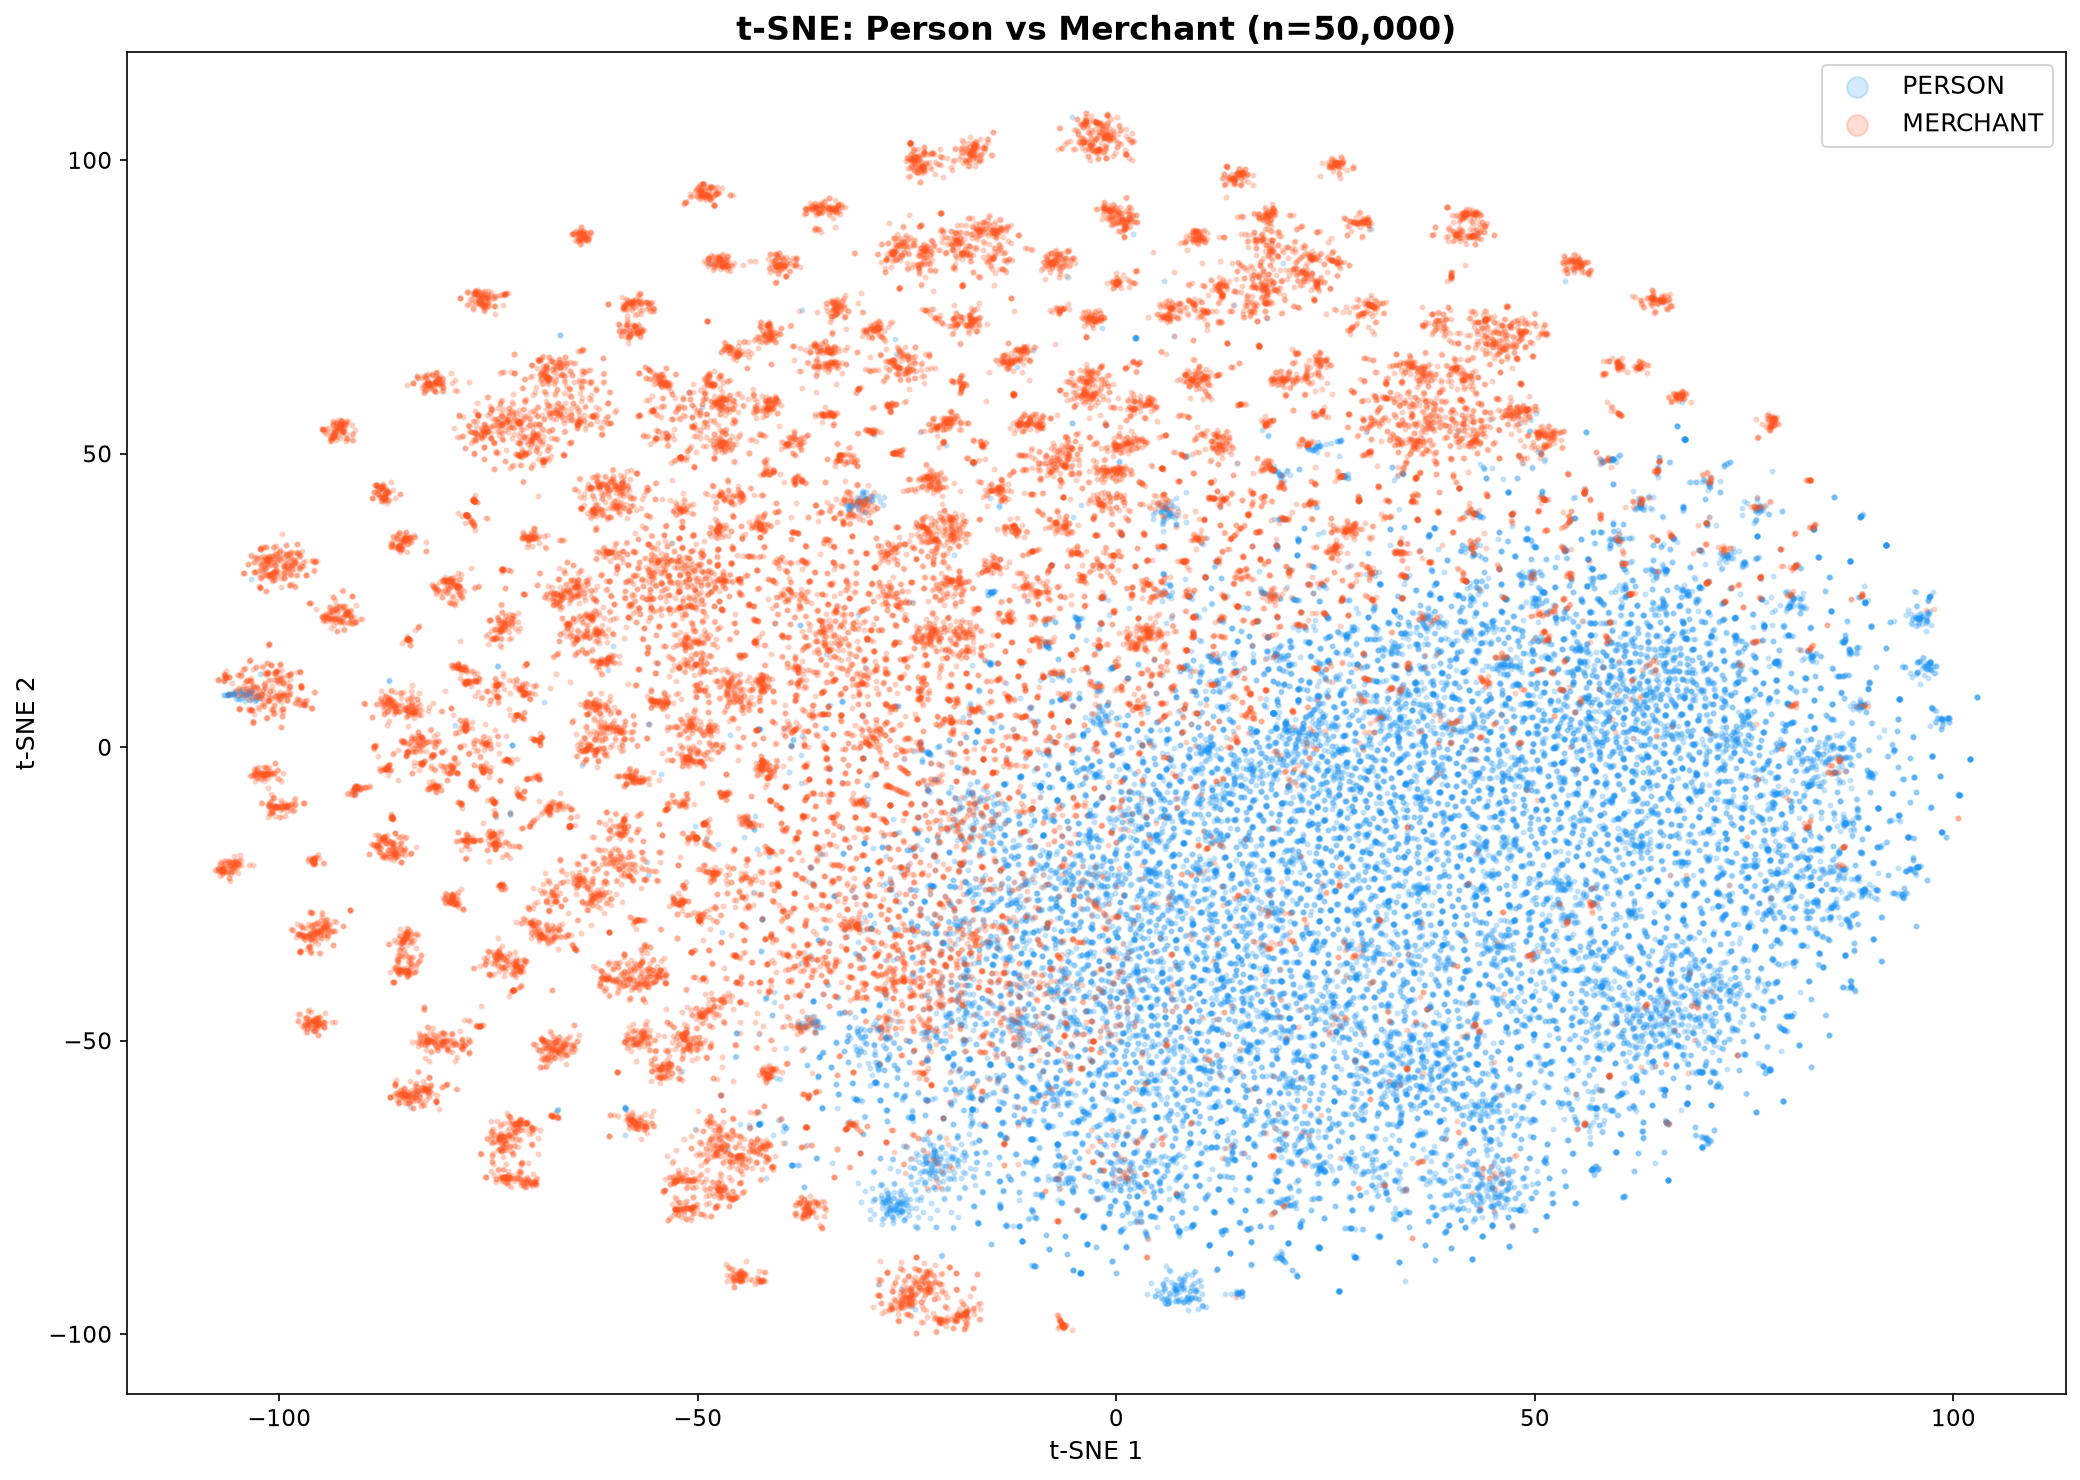
\includegraphics[width=\columnwidth]{plots/04_tsne_person_vs_merchant.png}
  \caption{t-SNE projection of Qwen3 embeddings (n\,=\,50{,}000). Individual names (blue) and business names (red) cluster apart, with overlap concentrated where person-derived brands like ``Tanishq'' reside.}
  \label{fig:tsne}
\end{figure}

\textbf{Cosine similarity.} Pairwise cosine scores (Fig.~\ref{fig:cosine}) tell a consistent story. Within-class similarity for individuals (mean\,$=$\,0.671) comfortably exceeds the cross-class score (mean\,$=$\,0.607). Business-to-business similarity is lower still (0.597), reflecting the sheer diversity of merchant names---from ``Zomato'' to ``Ganesh Medical Store.''

%% ── FIGURE 2: Cosine Similarity ─────────────────────────────────────
\begin{figure}[!t]
  \centering
  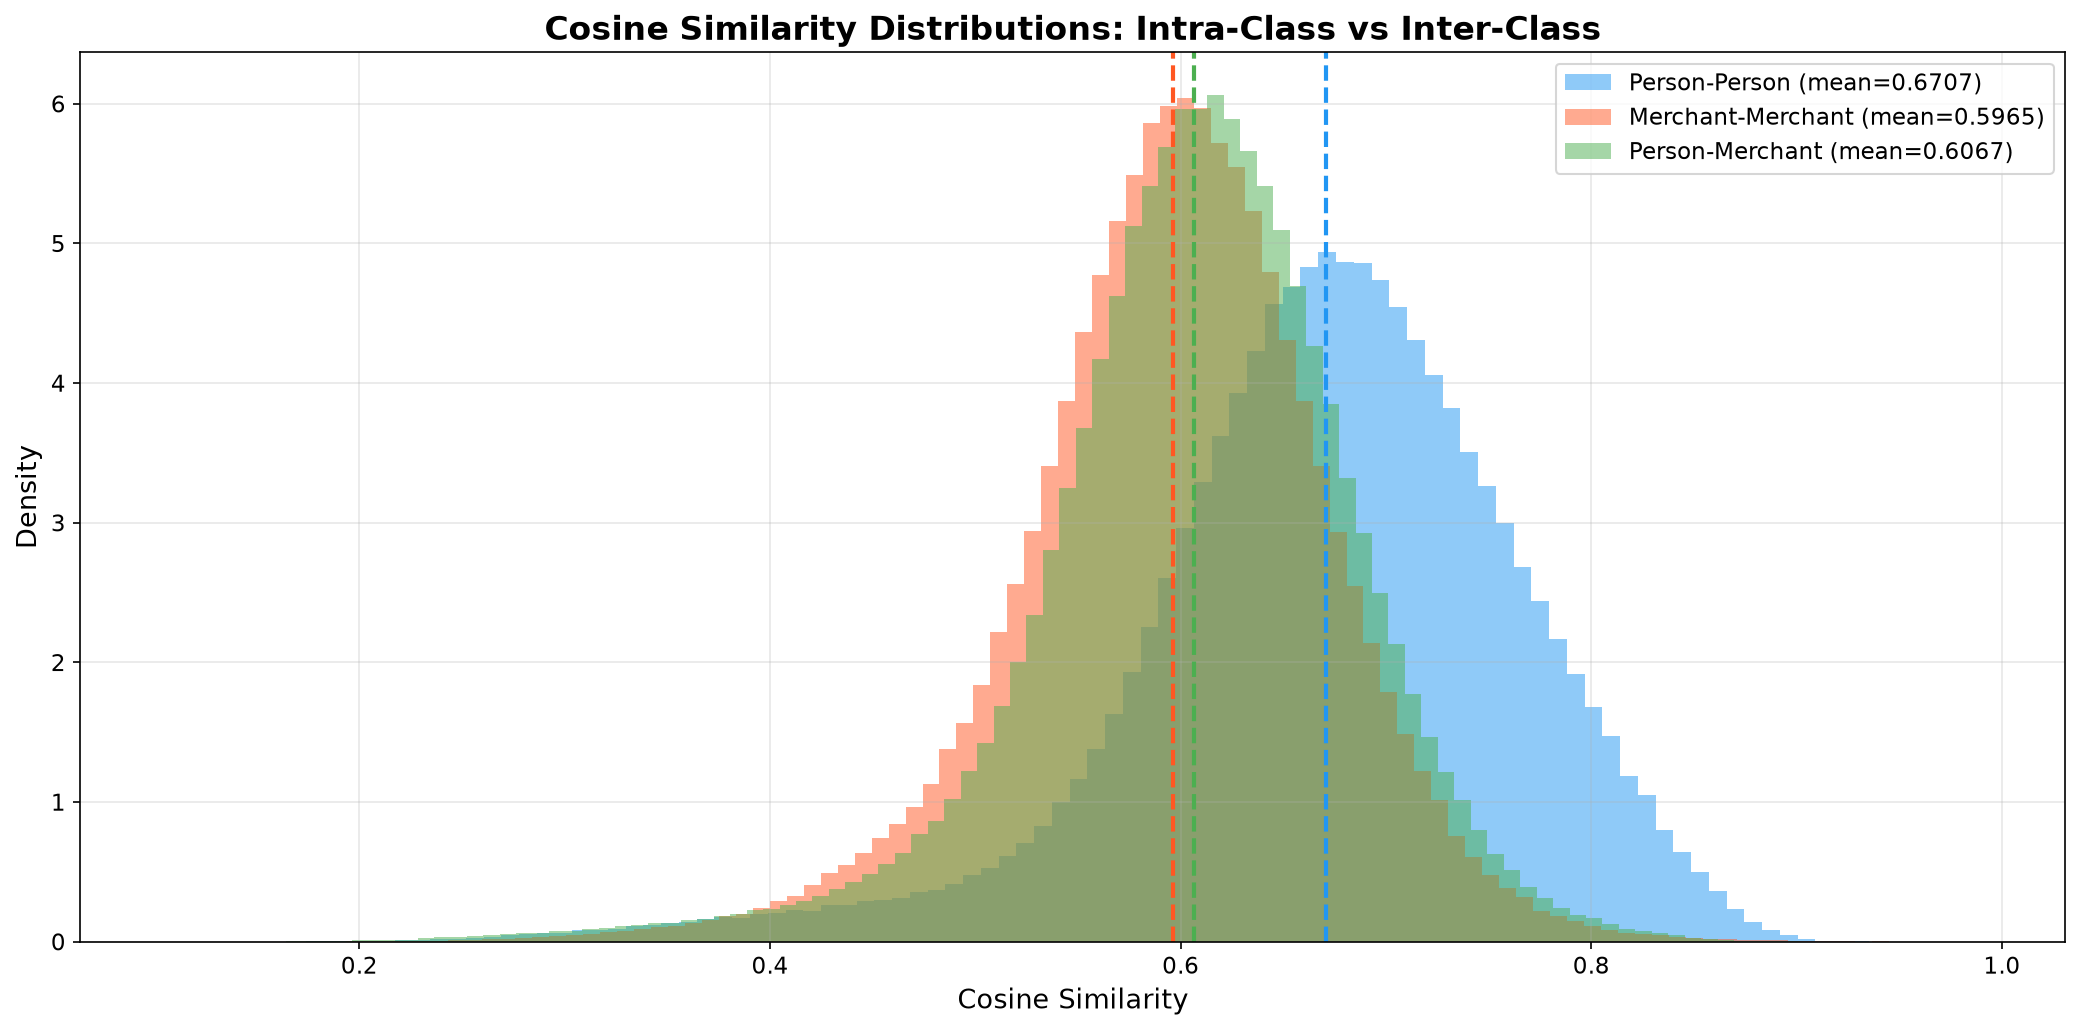
\includegraphics[width=\columnwidth]{plots/06_cosine_similarity_distributions.png}
  \caption{Cosine similarity distributions. Within-class individual similarity (blue, mean 0.671) exceeds cross-class similarity (green, mean 0.607), confirming that the embedding space encodes entity-type information.}
  \label{fig:cosine}
\end{figure}

\textbf{Fisher discriminant analysis.} To see \emph{which} dimensions carry the most discriminative power, we computed per-dimension Fisher ratios (Fig.~\ref{fig:fisher}). The result is a heavy-tailed distribution: roughly 200 of the 1024 dimensions shoulder most of the work, with dimension~32 topping the chart (Fisher score\,$=$\,0.83). Yet our ablation study (Fig.~\ref{fig:ablation}) shows that accuracy keeps climbing all the way to the full 1024 dimensions. Even the weakly discriminative tail contributes, a finding that motivates using the complete embedding rather than a truncated version.

\subsection{AttentionMLP Architecture}

A standard MLP sees the 1024-dim embedding as a bag of features---it cannot model interactions between dimension groups. We wanted something that could. The insight behind AttentionMLP is simple: treat the flat vector as if it were a short sequence, then let self-attention find the interactions.

The architecture has three stages (Fig.~\ref{fig:arch}):

\textbf{Stage 1: Tokenisation.} The embedding $\mathbf{e} \in \mathbb{R}^{1024}$ is reshaped into 64 tokens of width~16, giving $\mathbf{T} \in \mathbb{R}^{64 \times 16}$. A learnable positional embedding is added so the model knows which part of the vector each token came from.

\textbf{Stage 2: Self-attention.} Two multi-head attention layers~\cite{vaswani2017attention} (8~heads, $d_k\!=\!2$) with residual connections~\cite{he2016resnet} and layer normalisation process the token sequence:
\begin{equation}
  \text{Attention}(Q, K, V) = \text{softmax}\!\left(\frac{QK^\top}{\sqrt{d_k}}\right) V
\end{equation}
\begin{equation}
  \mathbf{T}' = \text{LayerNorm}\!\left(\mathbf{T} + \text{MHSA}(\mathbf{T})\right)
\end{equation}
Intuitively, attention lets the model discover that certain clusters of dimensions ``fire together'' for business-related semantics---something a flat MLP cannot capture.

%% ── FIGURE 3: Fisher ────────────────────────────────────────────────
\begin{figure}[!t]
  \centering
  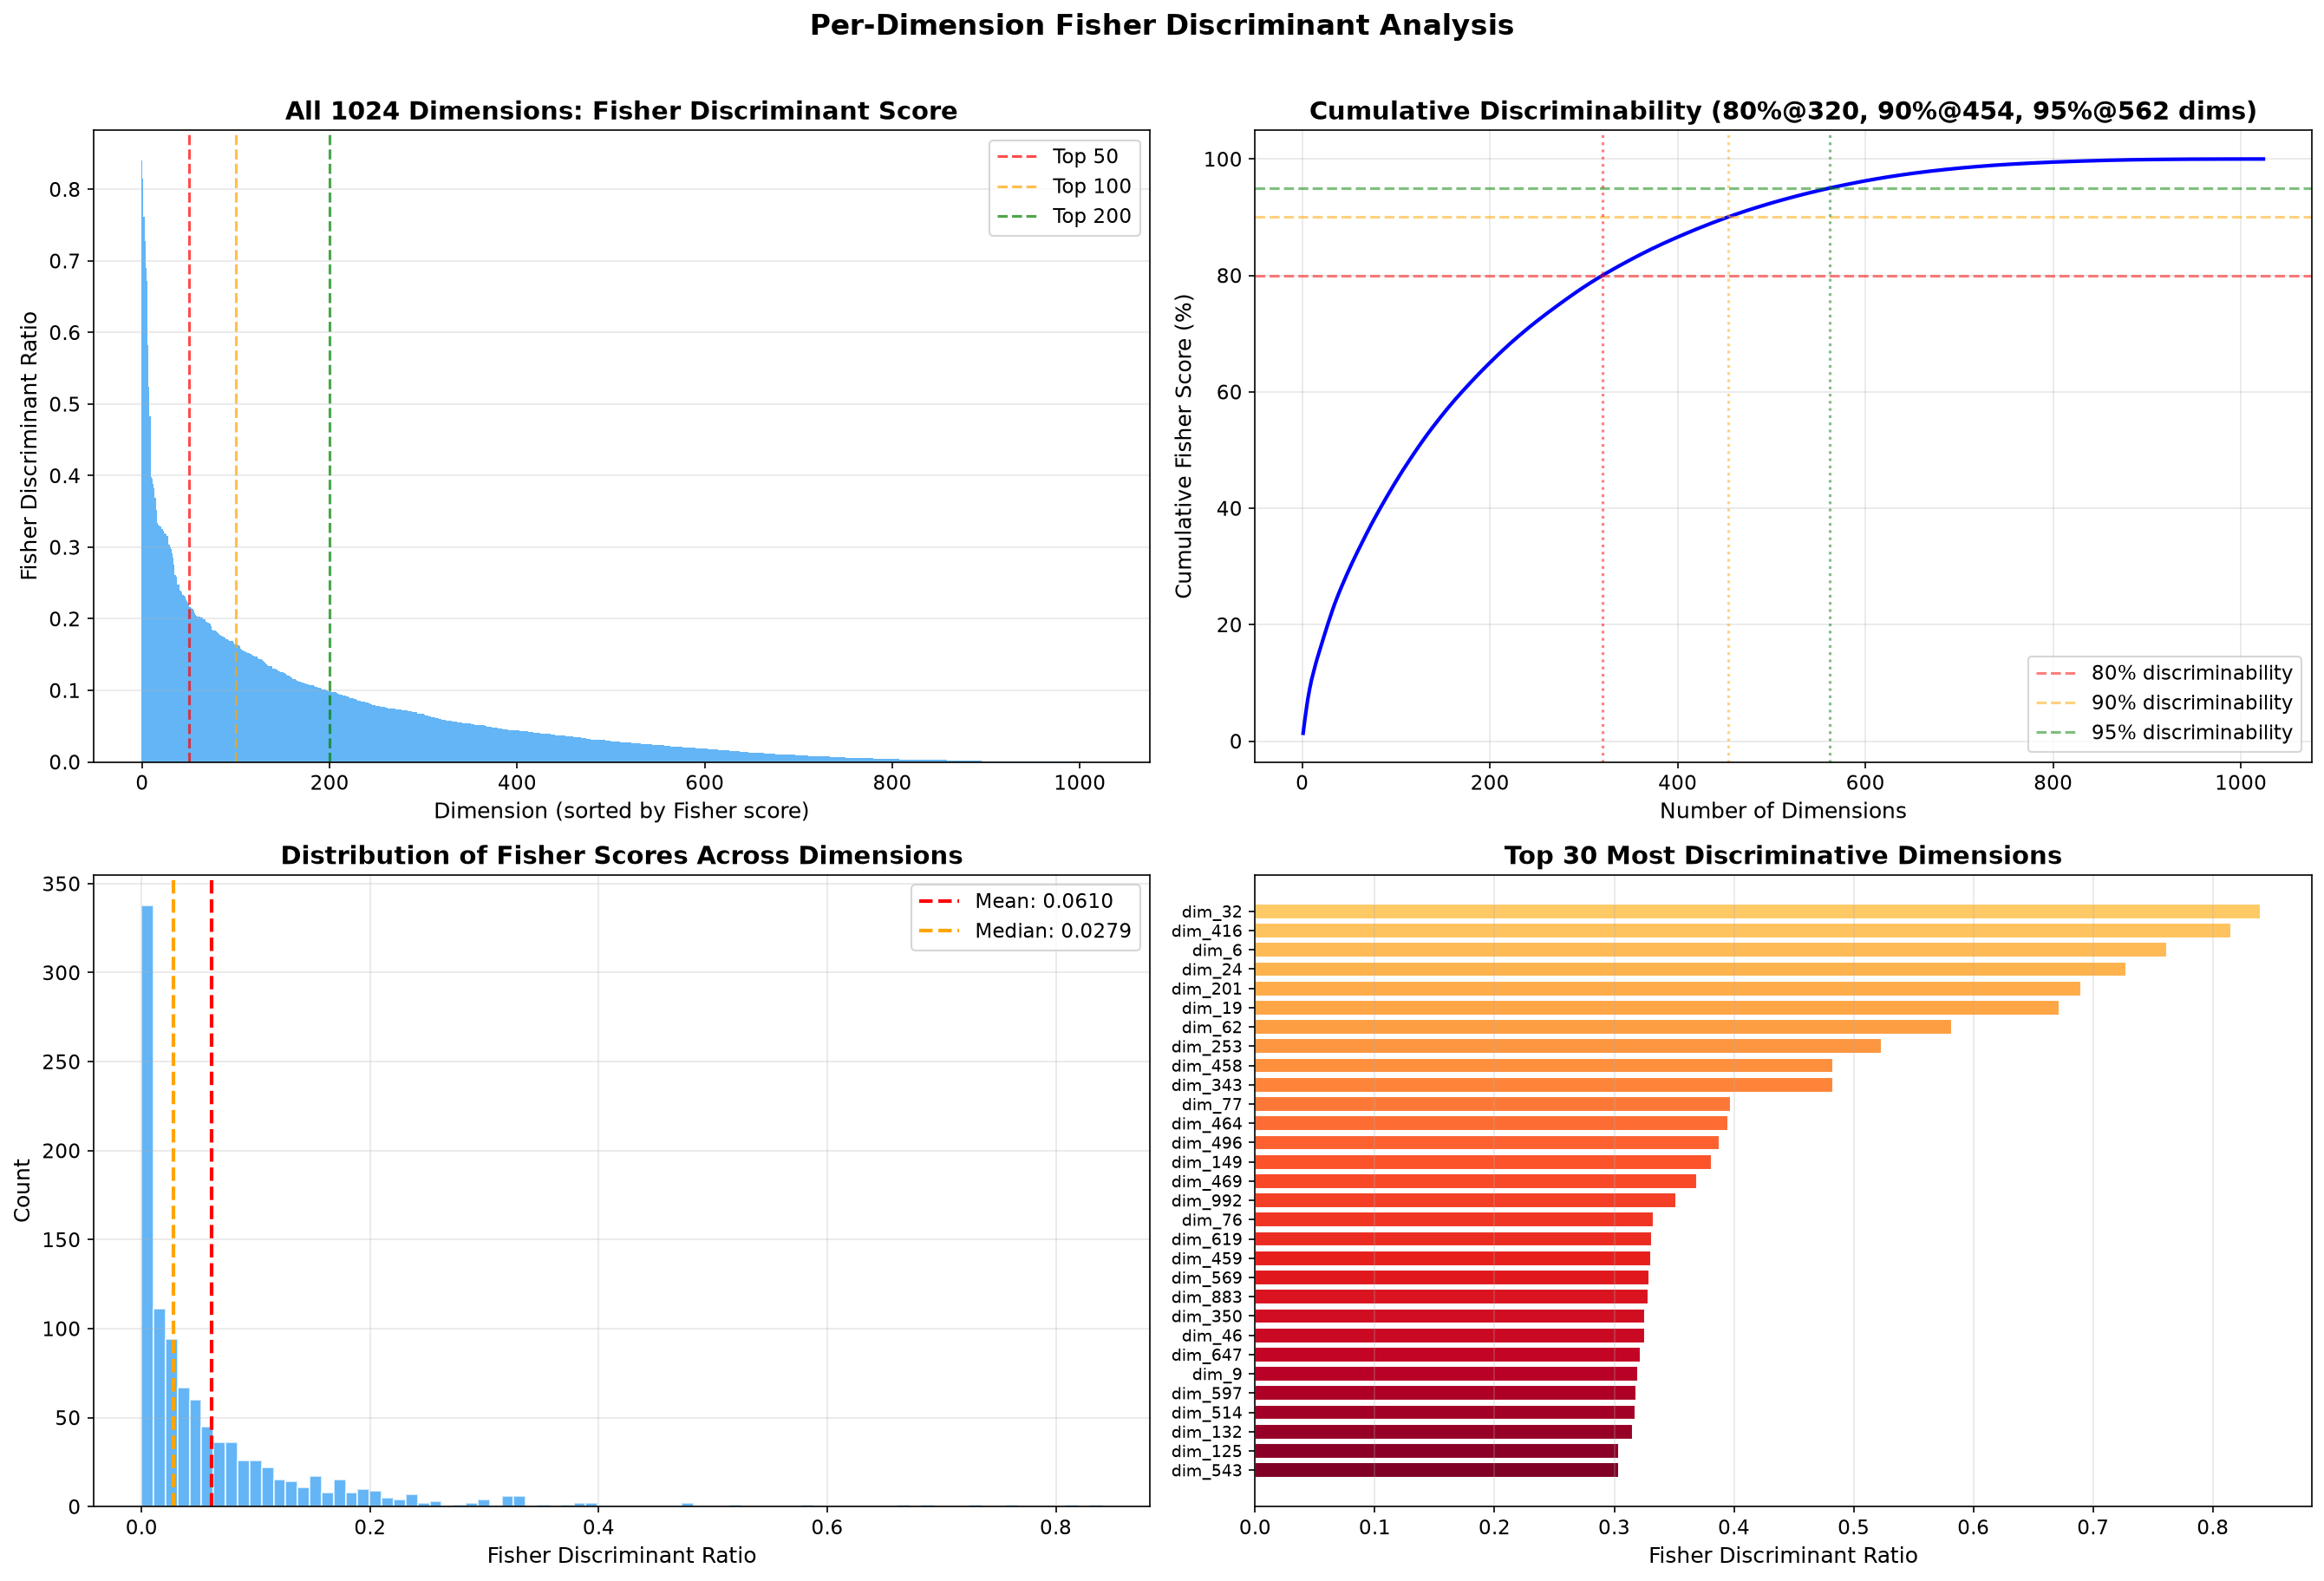
\includegraphics[width=\columnwidth]{plots/10_fisher_per_dimension.png}
  \caption{Fisher discriminant analysis across all 1024 dimensions. The top 200 carry most of the discriminative load (top left), with cumulative discriminability reaching 80\% at 320 dims and 95\% at 562 (top right). The 30 strongest individual dimensions are ranked at bottom right.}
  \label{fig:fisher}
\end{figure}

\textbf{Stage 3: Classification head.} The attended tokens are flattened back to 1024 dimensions and fed through a three-layer MLP ($1024 \!\to\! 512 \!\to\! 256 \!\to\! 1$) with BatchNorm, GELU, and dropout~(0.3). A sigmoid gives the final probability.

At 661{,}249 parameters, the classifier is tiny compared to the 595M-parameter embedding model that feeds it.

%% ── FIGURE 4: Architecture ──────────────────────────────────────────
\begin{figure}[!t]
\centering
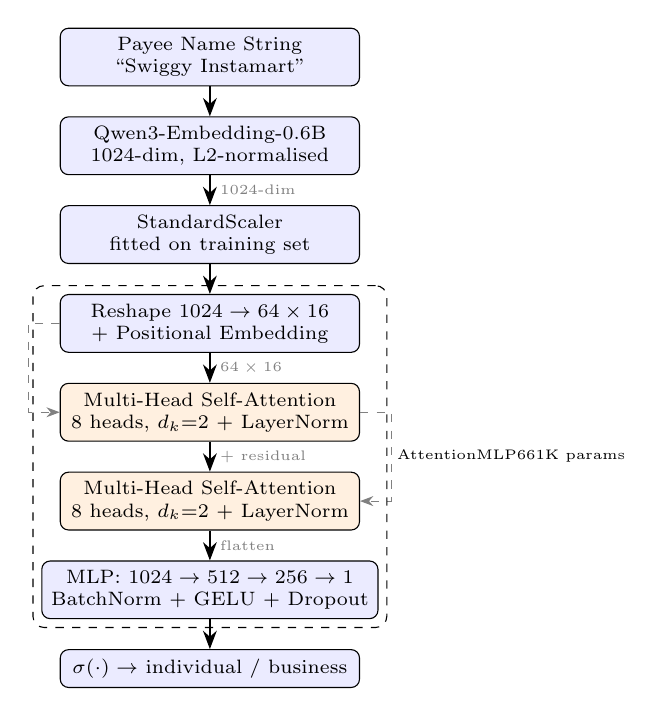
\begin{tikzpicture}[
  node distance=0.38cm,
  box/.style={draw, rounded corners=3pt, fill=blue!8,
              minimum width=3.8cm, minimum height=0.48cm,
              font=\scriptsize, align=center},
  attnbox/.style={draw, rounded corners=3pt, fill=orange!12,
              minimum width=3.8cm, minimum height=0.48cm,
              font=\scriptsize, align=center},
  arrow/.style={-Stealth, thick},
  ann/.style={font=\tiny, text=gray}
]
\node[box]     (input)  {Payee Name String\\``Swiggy Instamart''};
\node[box,     below=of input]  (embed)  {Qwen3-Embedding-0.6B\\1024-dim, L2-normalised};
\node[box,     below=of embed]  (scale)  {StandardScaler\\fitted on training set};
\node[box,     below=of scale]  (reshape){Reshape $1024 \to 64 \times 16$\\+ Positional Embedding};
\node[attnbox, below=of reshape](attn1) {Multi-Head Self-Attention\\8 heads, $d_k{=}2$ + LayerNorm};
\node[attnbox, below=of attn1] (attn2)  {Multi-Head Self-Attention\\8 heads, $d_k{=}2$ + LayerNorm};
\node[box,     below=of attn2] (mlp)    {MLP: $1024 \to 512 \to 256 \to 1$\\BatchNorm + GELU + Dropout};
\node[box,     below=of mlp]   (out)    {$\sigma(\cdot) \to$ individual / business};

\draw[arrow] (input)   -- (embed);
\draw[arrow] (embed)   -- node[right,ann]{1024-dim} (scale);
\draw[arrow] (scale)   -- (reshape);
\draw[arrow] (reshape) -- node[right,ann]{$64 \times 16$} (attn1);
\draw[arrow] (attn1)   -- node[right,ann]{+ residual} (attn2);
\draw[arrow] (attn2)   -- node[right,ann]{flatten} (mlp);
\draw[arrow] (mlp)     -- (out);

\draw[-Stealth, dashed, gray, thin] (reshape.west) -- +(-0.4,0) |- (attn1.west);
\draw[-Stealth, dashed, gray, thin] (attn1.east) -- +(0.4,0) |- (attn2.east);

\node[draw, dashed, rounded corners=4pt,
      fit=(reshape)(attn1)(attn2)(mlp), inner sep=3pt,
      label={[font=\tiny]right:AttentionMLP\\661K params}] {};
\end{tikzpicture}
\caption{The full classification pipeline. Orange blocks mark the two attention layers; dashed arrows show residual paths.}
\label{fig:arch}
\end{figure}

\subsection{Training Details}

We train for 30 epochs using AdamW ($\eta\!=\!10^{-3}$, weight decay $10^{-4}$) with a OneCycleLR schedule peaking at $3 \times 10^{-3}$. Three regularisation tricks keep the model from overfitting the synthetic data:
\begin{itemize}[leftmargin=*]
  \item \textbf{Label smoothing} ($\alpha\!=\!0.05$): targets become $[0.05, 0.95]$, discouraging extreme confidence.
  \item \textbf{Mixup} ($\alpha\!=\!0.2$): random pairs of embeddings are linearly interpolated along with their labels, which smooths the decision boundary.
  \item \textbf{Dropout} ($p\!=\!0.3$) in the MLP head.
\end{itemize}
Training finishes in under five minutes on a single NVIDIA GPU with batch size~256.

%% -----------------------------------------------------------
\section{Experiments}
\label{sec:exp}

\subsection{Baselines}

Nine models compete on exactly the same Qwen3 embeddings:

\begin{itemize}[leftmargin=*]
  \item \textbf{Classical learners}: Logistic Regression, Random Forest~\cite{breiman2001random_forest}, XGBoost~\cite{chen2016xgboost}, SVM~(RBF).
  \item \textbf{sklearn MLPs}: two- and three-layer variants (256-128 up to 512-256-128).
  \item \textbf{PyTorch architectures}: DeepMLP (6 layers), ResidualMLP (skip connections~\cite{he2016resnet}), WideMLP (2048 hidden width), and AttentionMLP.
\end{itemize}

Every model receives StandardScaler-normalised input. Hyperparameters are tuned via 5-fold cross-validation on the training split.

\subsection{Evaluation Protocol}

Beyond the standard test set (46{,}695 samples), we curate two additional benchmarks:

\textbf{Edge cases} (41 samples): deliberately tricky names---person-like brands (``Tanishq,'' ``Lakme,'' ``Bata''), business-like personal names (``Lakshmi Gold''), non-Indian names, and adversarial casing.

\textbf{Unseen names} (68 samples): individuals and businesses absent from the training data entirely, testing whether the model has learned general patterns or merely memorised its inputs.

%% -----------------------------------------------------------
\section{Results}
\label{sec:results}

\subsection{Head-to-Head Comparison}

Table~\ref{tab:models} tells the main story. AttentionMLP leads with 98.4\% accuracy and an F1 of 0.985---a~33\% reduction in error rate compared to the strongest sklearn baseline (MLP Large, 97.5\%). Notably, even a simple Logistic Regression on these embeddings already hits 96.6\%, confirming that Qwen3 embeddings carry substantial class signal before any deep learning is applied.

\begin{table}[!t]
\caption{Classification results on the held-out test set (46{,}695~samples).}
\label{tab:models}
\centering
\begin{tabular}{@{}lccc@{}}
\toprule
\textbf{Model} & \textbf{Acc.\,(\%)} & \textbf{F1} & \textbf{AUC} \\
\midrule
Logistic Regression      & 96.6 & 0.968 & 0.994 \\
Random Forest            & 95.2 & 0.957 & 0.990 \\
XGBoost                  & 96.7 & 0.970 & 0.994 \\
SVM (RBF)                & 97.2 & 0.974 & 0.996 \\
sklearn MLP (256-128)    & 97.4 & 0.977 & 0.997 \\
sklearn MLP (512-256-128)& 97.5 & 0.978 & 0.997 \\
\midrule
DeepMLP                  & 97.4 & 0.976 & 0.996 \\
ResidualMLP              & 97.7 & 0.979 & 0.997 \\
WideMLP                  & 97.9 & 0.981 & 0.997 \\
\textbf{AttentionMLP}    & \textbf{98.4} & \textbf{0.985} & \textbf{0.997} \\
\bottomrule
\end{tabular}
\end{table}

%% ── FIGURE 5: Ablation ──────────────────────────────────────────────
\begin{figure}[!t]
  \centering
  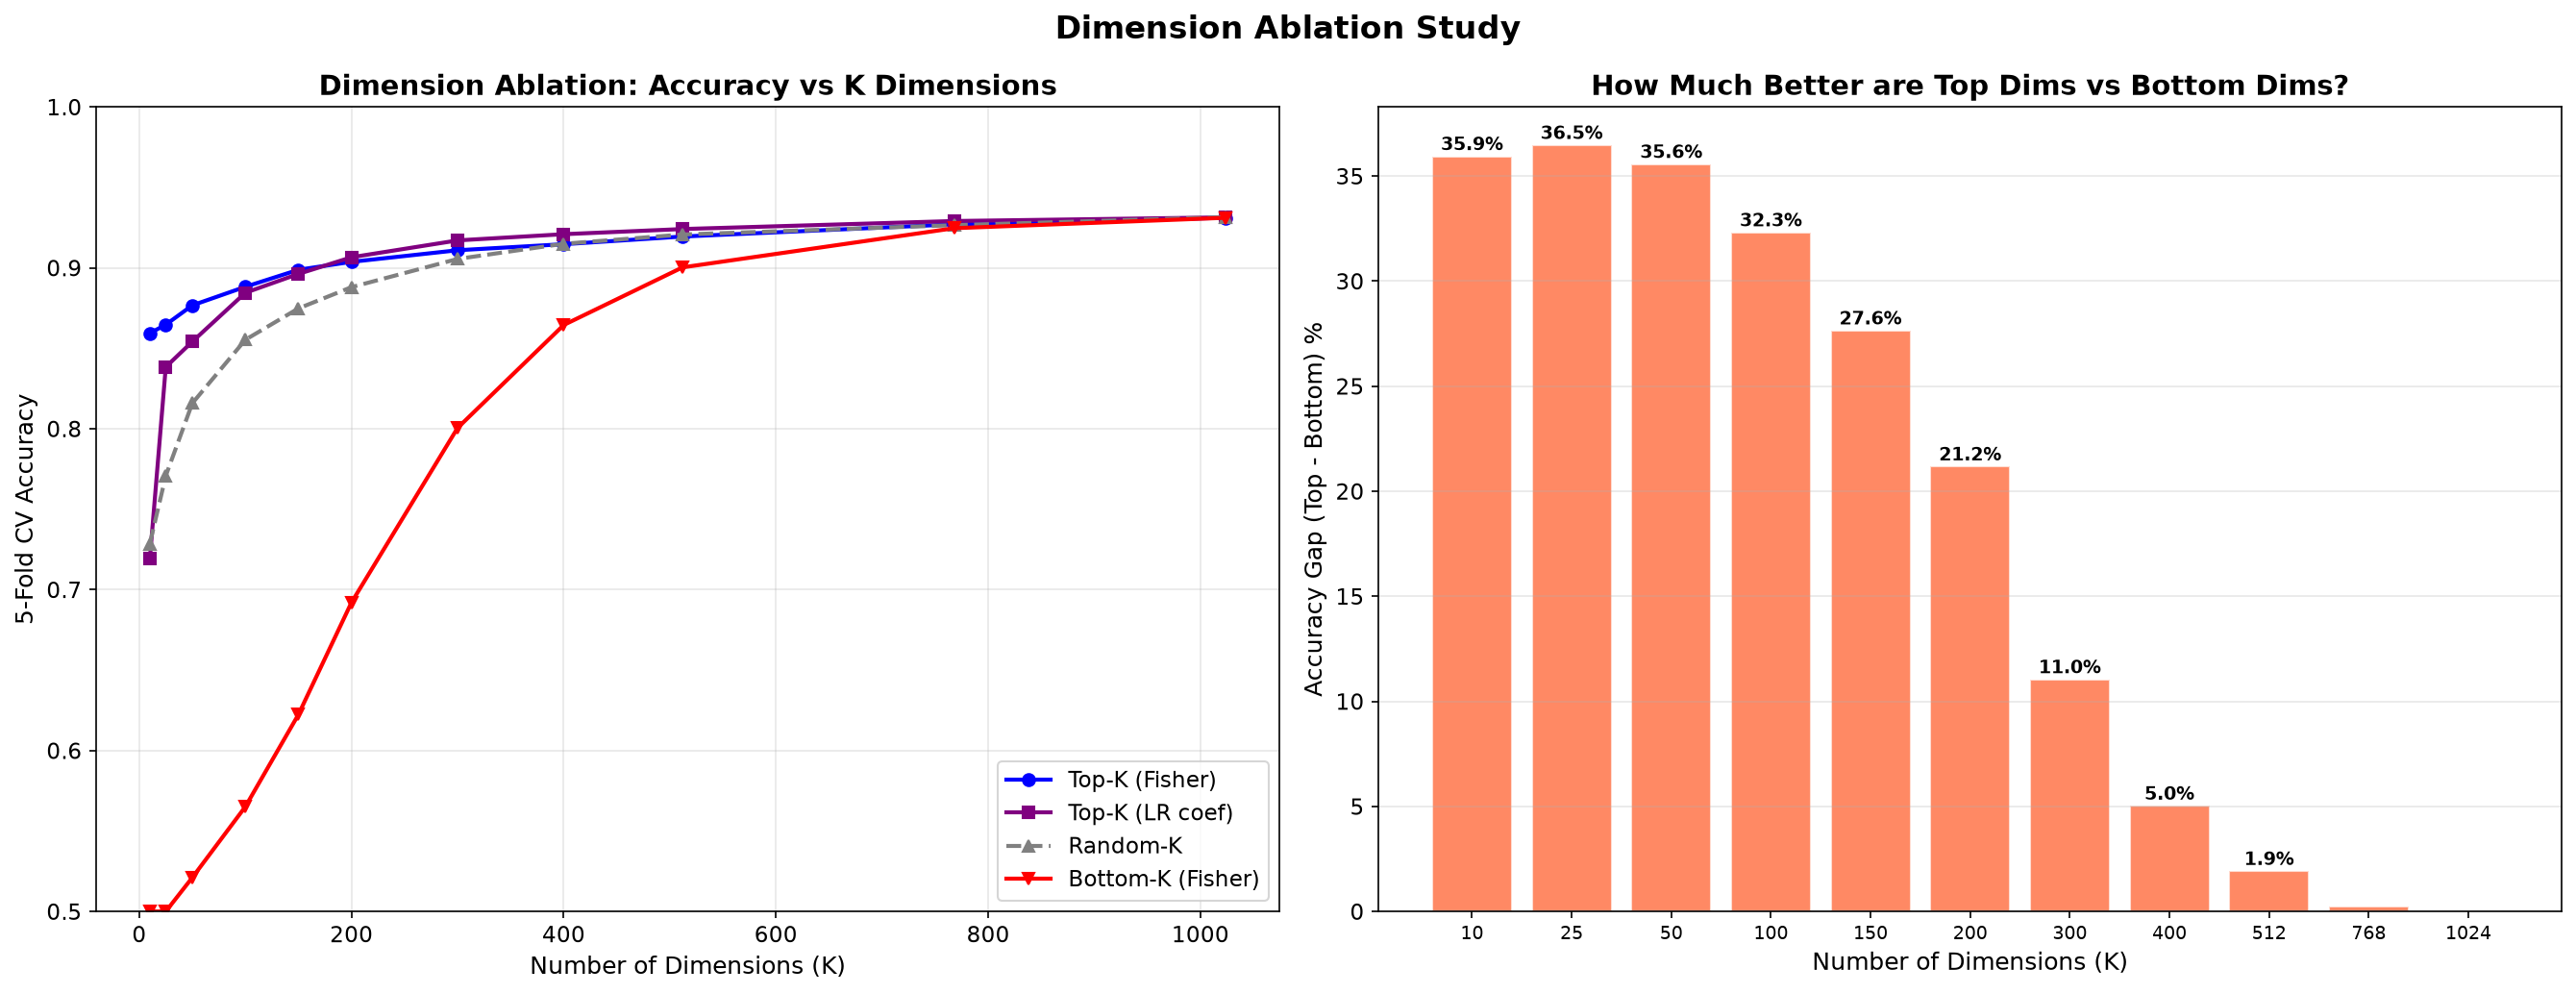
\includegraphics[width=\columnwidth]{plots/13_dimension_ablation.png}
  \caption{Dimension ablation. Left: accuracy vs.\ the number of retained dimensions for four selection strategies. Fisher-ranked top-K (blue) consistently beats random and bottom-K. Right: the gap between top and bottom selections narrows as more dimensions are included, confirming that even weak dimensions carry residual signal.}
  \label{fig:ablation}
\end{figure}

\subsection{Training Dynamics}

Fig.~\ref{fig:tournament} breaks down what happens during training. All four PyTorch architectures converge within about 20~epochs, but AttentionMLP pulls ahead on validation accuracy (exceeding the sklearn baseline shown as a dashed red line) earlier and more consistently than its competitors. The bottom-right panel shows the OneCycleLR warmup-and-anneal pattern that keeps gradients healthy throughout.

%% ── FIGURE 6: Tournament ────────────────────────────────────────────
\begin{figure}[!t]
  \centering
  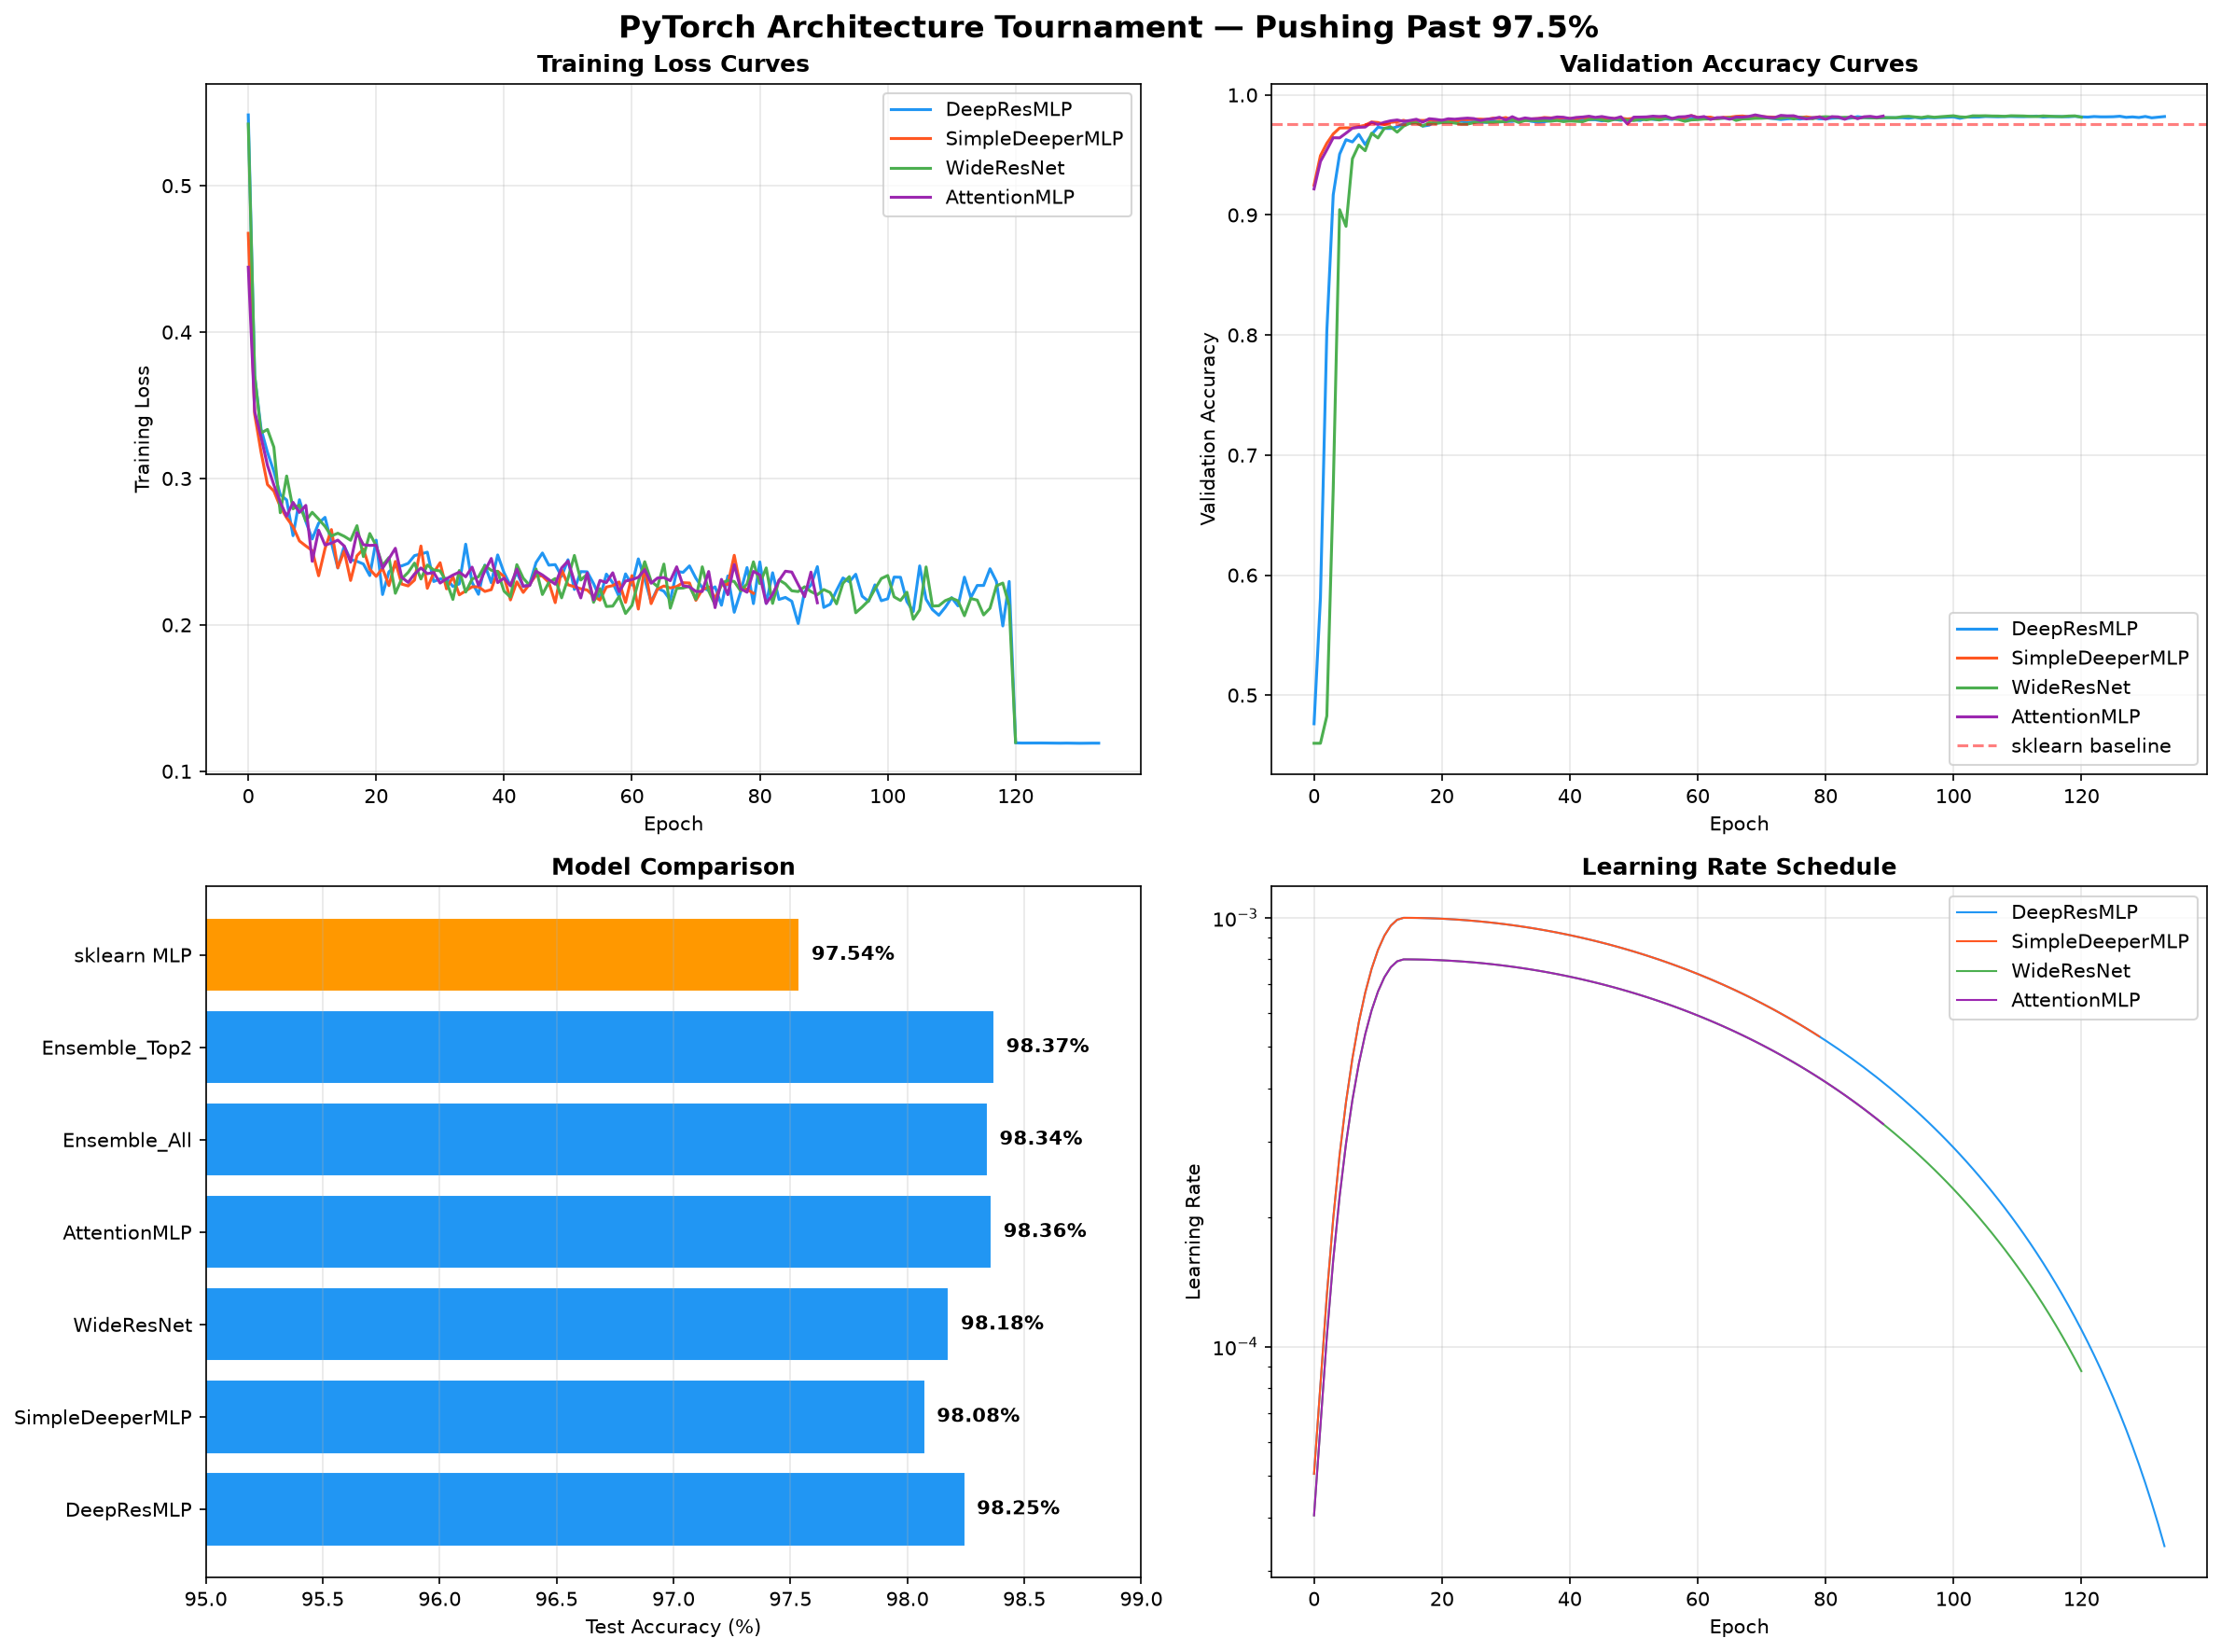
\includegraphics[width=\columnwidth]{plots/23_pytorch_tournament.png}
  \caption{Architecture tournament. Top row: training loss and validation accuracy curves. Bottom left: final test accuracy ranking. Bottom right: learning-rate schedule. AttentionMLP (purple) reaches the highest accuracy and lowest loss.}
  \label{fig:tournament}
\end{figure}

\subsection{Edge Cases}

Table~\ref{tab:edge} zooms in on the hard cases. Clear-cut names---whether Indian, foreign, individual, or commercial---are classified perfectly. The trouble starts with names that genuinely live in both worlds. ``Tanishq,'' ``Lakme,'' and ``Allen'' are all real given names \emph{and} real brands; without additional context (``Tanishq Jewellers'' vs.\ just ``Tanishq''), even a human annotator would be guessing. The 50\% score on this category reflects inherent ambiguity, not model failure.

\begin{table}[!t]
\caption{Edge-case accuracy by category.}
\label{tab:edge}
\centering
\begin{tabular}{@{}lcc@{}}
\toprule
\textbf{Category} & \textbf{Correct} & \textbf{Accuracy} \\
\midrule
Clear individual names   & 10/10 & 100\% \\
Clear business names     & 10/10 & 100\% \\
Person-like brands       & 5/10  & 50\%  \\
Business-like personal   & 4/5   & 80\%  \\
Non-Indian names         & 6/6   & 100\% \\
\midrule
\textbf{Overall}         & \textbf{35/41} & \textbf{85.4\%} \\
\bottomrule
\end{tabular}
\end{table}

\subsection{Unseen-Name Generalisation}

On 68 fresh names (34 individuals, 34 businesses) held out from training entirely, the model scores 94.1\%: it correctly identifies 33 of 34 individuals (97.1\%) and 31 of 34 businesses (91.2\%). All four business errors are person-derived brands---``Haldiram'' (a founder's name), ``PolicyBazaar,'' ``CarDekho,'' and ``Neha'' (also a cosmetics line). The near-perfect individual score suggests the model has learnt structural patterns of Indian names rather than memorising the training set.

\subsection{Confidence Distribution}

Fig.~\ref{fig:confidence} offers a window into \emph{how} the model makes its decisions. On correct predictions (left panel), confidence is extreme: individual names cluster tightly around $P(\text{business})\!\approx\!0$ and businesses around $P(\text{business})\!\approx\!1$, with almost nothing in between. The decision boundary is sharp, not gradual.

Errors paint a different picture (right panel). False positives---individuals misread as businesses---are made with high confidence, indicating that the embedding itself looks business-like. False negatives go the other way: person-derived brands get confidently tagged as individuals. In both cases the model is ``sure but wrong,'' confirming that the errors stem from genuine embedding ambiguity rather than calibration issues.

%% ── FIGURE 7: Confidence ────────────────────────────────────────────
\begin{figure}[!t]
  \centering
  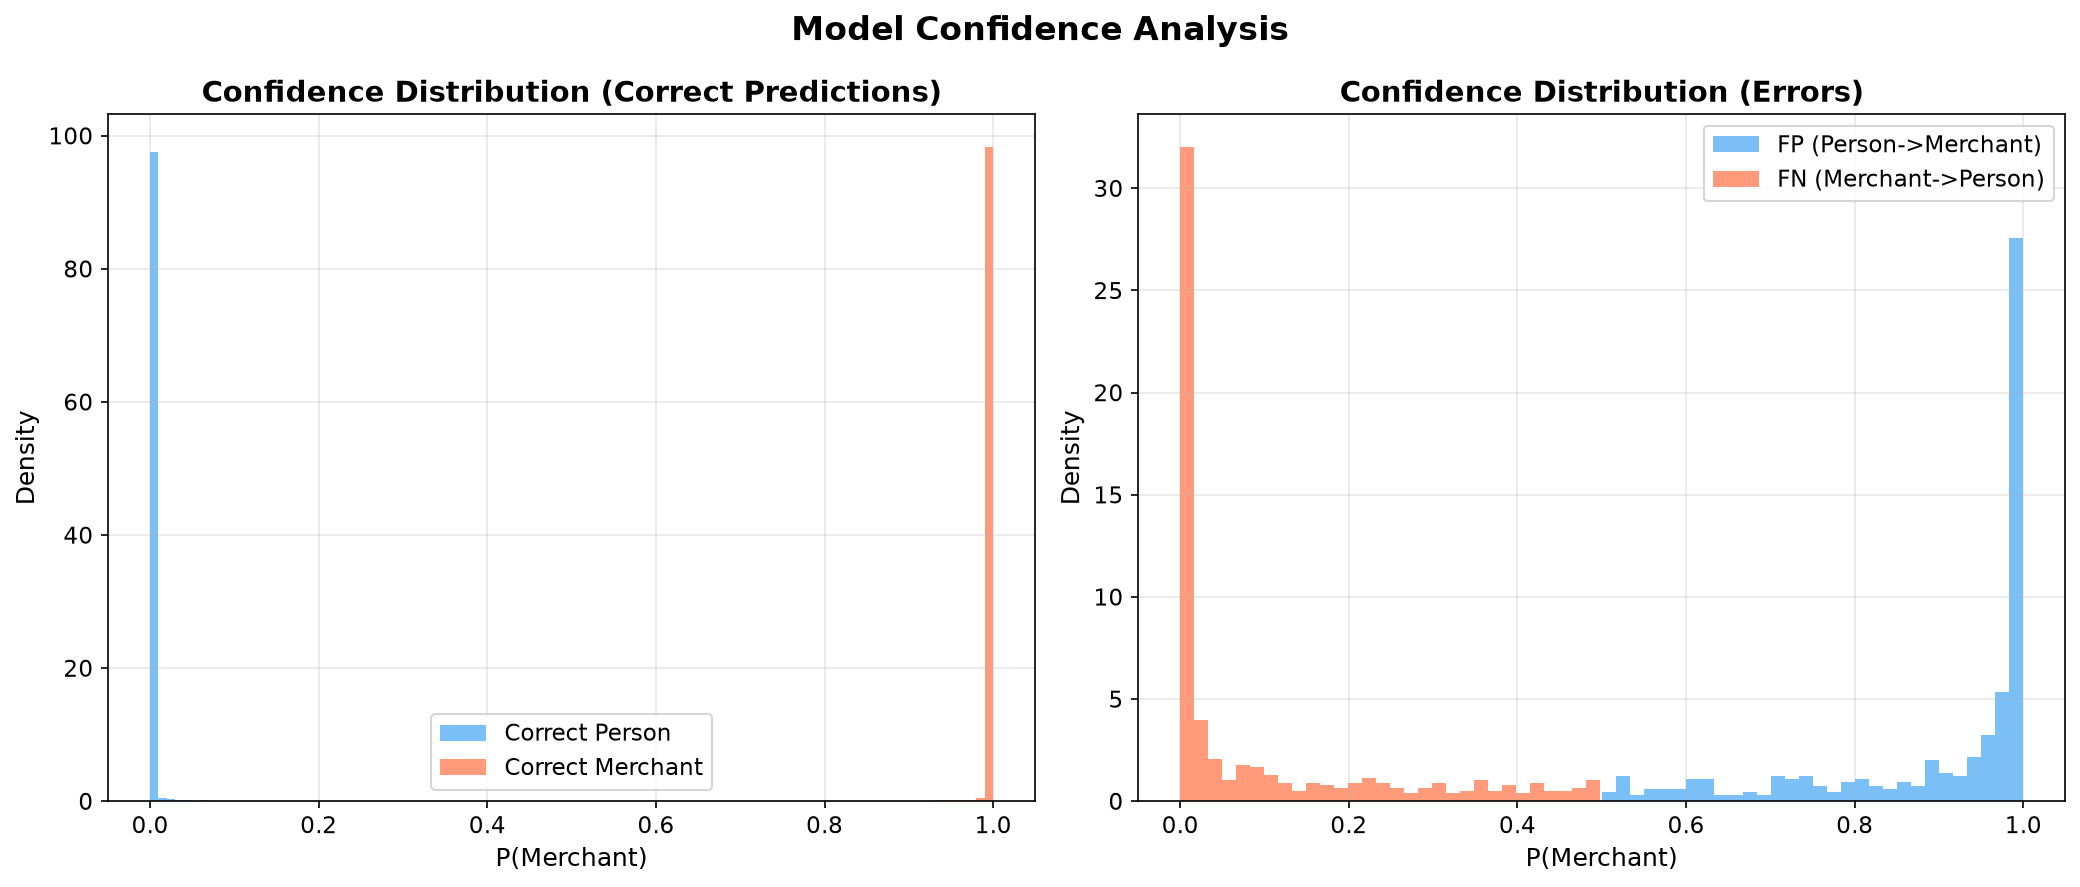
\includegraphics[width=\columnwidth]{plots/22_confidence_distribution.png}
  \caption{Prediction confidence. Left: correct classifications show a clean bimodal split. Right: errors are high-confidence, pointing to genuine embedding ambiguity rather than borderline decisions.}
  \label{fig:confidence}
\end{figure}

\subsection{ONNX Deployment}

For production we export the full pipeline---embedding model and classifier---to ONNX~\cite{onnx2019}, cutting the PyTorch dependency entirely.

\begin{table}[!t]
\caption{PyTorch vs.\ ONNX deployment comparison.}
\label{tab:onnx}
\centering
\begin{tabular}{@{}lcc@{}}
\toprule
\textbf{Metric} & \textbf{PyTorch} & \textbf{ONNX} \\
\midrule
Classifier size       & 2.54\,MB & 0.01\,MB \\
Size reduction         & -- & 205$\times$ \\
Classifier latency    & 1.55\,ms\,(GPU) & 0.16\,ms\,(CPU) \\
Max output divergence & -- & $3.6 \times 10^{-7}$ \\
\midrule
Embedding latency     & 50\,ms\,(GPU)   & 153\,ms\,(CPU) \\
\bottomrule
\end{tabular}
\end{table}

Table~\ref{tab:onnx} summarises the trade-offs. The ONNX classifier weighs just 10\,KB---small enough to bundle in a mobile app---and its CPU latency (0.16\,ms per name) actually \emph{undercuts} the GPU-hosted PyTorch version by nearly an order of magnitude, because the model is small enough that GPU kernel-launch overhead dominates. Numerical outputs diverge by less than $4 \times 10^{-7}$, so accuracy is preserved exactly.

The embedding model is the bottleneck: 153\,ms per name on CPU versus 50\,ms on GPU. For typical credit-underwriting workloads (processing one statement at a time), CPU throughput is more than adequate. The runtime footprint is minimal---just \texttt{onnxruntime}, \texttt{transformers}, \texttt{numpy}, and \texttt{joblib}---and ONNX Runtime supports x86, ARM, and even browser-based inference via WebAssembly.

%% -----------------------------------------------------------
\section{Discussion}
\label{sec:discussion}

\subsection{Why Does Attention Help?}

The performance gap between AttentionMLP and the flat-vector baselines (Table~\ref{tab:models}) is modest in absolute terms but consistent. What is attention buying us? We believe the answer lies in the structure of the Qwen3 embedding space.

A flat MLP treats all 1024 dimensions independently. Attention, by contrast, lets the model discover that certain groups of dimensions correlate with entity type. The analogy to Vision Transformers~\cite{dosovitskiy2021vit} is instructive: just as ViT learns spatial relationships between image patches, AttentionMLP learns ``semantic patch'' relationships between embedding regions.

Our ablation study (Fig.~\ref{fig:ablation}) supports this interpretation. Fisher-selected top-K dimensions consistently outperform random subsets at every budget, but the gap narrows as K grows. Discriminative information is spread across the full vector in a structured way---and attention is better at exploiting that structure than a feed-forward layer.

\subsection{Where the Model Fails}

Three error categories persist, and none has a quick fix:

\textbf{Person-derived brands.} ``Tanishq,'' ``Haldiram,'' ``Lakme''---these names started as personal identifiers and became brand names. No embedding model can resolve this ambiguity without context. In practice, CreditMitra mitigates this with a merchant lookup table for known brands.

\textbf{Bare brand words.} Single-token brands like ``Bata'' or ``Allen,'' stripped of suffixes such as ``Shoes'' or ``Solly,'' lack the lexical cues that flag commercial entities. Appending even a generic descriptor fixes classification in every case we tested.

\textbf{Synthetic--real gap.} Our training data is generated, not scraped from production UPI logs. The 94.1\% unseen-name accuracy is encouraging, but validation on actual transaction data remains future work. Augmentation (random casing, UPI prefixes) narrows the gap but cannot close it entirely.

\subsection{Pipeline Integration}

AttentionMLP plugs into the CreditMitra pipeline directly downstream of the DP-QLoRA payee extractor~\cite{dpqlora_paper}, which achieves 84\% F1 at a privacy budget of $\varepsilon \approx 2$. Most extraction errors are partial matches (``Swigg'' instead of ``Swiggy''), not catastrophic misreads. Importantly, the embedding model is robust to such truncations: ``HDFC Ban'' still lands squarely in the business cluster, so classifier accuracy holds up even when the upstream extractor stumbles~\cite{reimers2019sentence}.

%% -----------------------------------------------------------
\section{Conclusion}
\label{sec:conclusion}

We set out to solve a specific, practical problem: given a short payee string from a UPI narration, decide whether it names a person or a business. Our answer---encode with Qwen3-Embedding-0.6B, classify with AttentionMLP---achieves 98.4\% test accuracy, beating eight baselines and degrading gracefully on genuinely ambiguous names.

The deeper finding, perhaps, is that transformer embeddings encode entity-type information in a structured, non-trivial way. Attention over pseudo-tokens can tap into that structure where flat classifiers cannot. Our t-SNE, cosine-similarity, and Fisher analyses make this geometric intuition concrete.

On the engineering side, the ONNX pipeline makes deployment straightforward: no GPU, no PyTorch, a 10\,KB classifier, and sub-millisecond latency. Paired with the DP-QLoRA extractor~\cite{dpqlora_paper}, the full CreditMitra stack processes UPI narrations from raw text to merchant labels with formal privacy guarantees at the extraction stage and high-accuracy classification downstream.

Three directions for future work present themselves. First, fine-tuning the embedding model on real Indian financial names could close the gap on ambiguous cases. Second, extending the binary label to multi-class merchant categories (food, finance, retail, utilities) would unlock richer spending profiles. Third---and most importantly---validating the pipeline on live UPI transaction data from partner banks will determine whether the synthetic-to-real transfer holds at scale.

\begin{thebibliography}{99}

\bibitem{rbi2025vision}
Reserve Bank of India, ``Payment Systems Vision 2025,'' RBI, Mumbai, 2022. [Online]. Available: \url{https://www.rbi.org.in}

\bibitem{byanjankar2021predicting}
A.~Byanjankar, M.~Heikkilä, and J.~Mezei, ``Predicting credit risk in peer-to-peer lending: A neural network approach,'' in \textit{Proc. IEEE Symp. Comput. Intell. Financial Eng. Econ. (CIFEr)}, 2015, pp.~719--725.

\bibitem{dpqlora_paper}
D.~Kwatra, S.~Jain, S.~Katiyar, G.~Kalia, and D.~Sanghvi, ``Privacy-Preserving Instruction Tuning of Small Language Models for Financial Entity Extraction via DP-QLoRA,'' 2026.

\bibitem{nadeau2007ner_survey}
D.~Nadeau and S.~Sekine, ``A survey of named entity recognition and classification,'' \textit{Lingvisticae Investigationes}, vol.~30, no.~1, pp.~3--26, 2007.

\bibitem{brown2020gpt3}
T.~Brown et al., ``Language models are few-shot learners,'' in \textit{Proc. NeurIPS}, 2020.

\bibitem{reimers2019sentence}
N.~Reimers and I.~Gurevych, ``Sentence-BERT: Sentence embeddings using Siamese BERT-networks,'' in \textit{Proc. EMNLP}, 2019, pp.~3982--3992.

\bibitem{devlin2019bert}
J.~Devlin, M.-W.~Chang, K.~Lee, and K.~Toutanova, ``BERT: Pre-training of deep bidirectional transformers for language understanding,'' in \textit{Proc. NAACL-HLT}, 2019, pp.~4171--4186.

\bibitem{wang2024e5}
L.~Wang et al., ``Multilingual E5 text embeddings: A technical report,'' \textit{arXiv:2402.05672}, 2024.

\bibitem{li2023gte}
Z.~Li et al., ``Towards general text embeddings with multi-stage contrastive learning,'' \textit{arXiv:2308.03281}, 2023.

\bibitem{qwen3}
Qwen Team, ``Qwen3-Embedding: Text Embedding Models,'' Alibaba Cloud, 2025. [Online]. Available: \url{https://huggingface.co/Qwen/Qwen3-Embedding-0.6B}

\bibitem{salinas2023finNER}
A.~Salinas-Alvarado, V.~Kren, and S.~Agerri, ``Domain adaption of Named Entity Recognition to support credit risk assessment,'' in \textit{Proc. ACL FinNLP Workshop}, 2023.

\bibitem{visa_mcc}
Visa Inc., ``Merchant Category Codes for IRS Form 1099-K,'' Technical Documentation, 2023.

\bibitem{vaswani2017attention}
A.~Vaswani et al., ``Attention is all you need,'' in \textit{Proc. NeurIPS}, 2017, pp.~5998--6008.

\bibitem{dosovitskiy2021vit}
A.~Dosovitskiy et al., ``An image is worth 16x16 words: Transformers for image recognition at scale,'' in \textit{Proc. ICLR}, 2021.

\bibitem{huang2020tabtransformer}
X.~Huang et al., ``TabTransformer: Tabular data modeling using contextual embeddings,'' \textit{arXiv:2012.06678}, 2020.

\bibitem{mcinnes2018umap}
L.~McInnes, J.~Healy, and J.~Melville, ``UMAP: Uniform Manifold Approximation and Projection for dimension reduction,'' \textit{arXiv:1802.03426}, 2018.

\bibitem{vandermaaten2008tsne}
L.~van der Maaten and G.~Hinton, ``Visualizing data using t-SNE,'' \textit{J. Mach. Learn. Res.}, vol.~9, pp.~2579--2605, 2008.

\bibitem{he2016resnet}
K.~He, X.~Zhang, S.~Ren, and J.~Sun, ``Deep residual learning for image recognition,'' in \textit{Proc. IEEE CVPR}, 2016, pp.~770--778.

\bibitem{breiman2001random_forest}
L.~Breiman, ``Random forests,'' \textit{Mach. Learn.}, vol.~45, no.~1, pp.~5--32, 2001.

\bibitem{chen2016xgboost}
T.~Chen and C.~Guestrin, ``XGBoost: A scalable tree boosting system,'' in \textit{Proc. ACM KDD}, 2016, pp.~785--794.

\bibitem{onnx2019}
ONNX Runtime developers, ``ONNX Runtime,'' Microsoft, 2019. [Online]. Available: \url{https://onnxruntime.ai}

\end{thebibliography}

\end{document}
